\section{Conclusion}
\label{sec:conclusion}

\subsection{Overall Analysis}
\label{sec:conclusion: Overall Analysis}
From our data analysis and the graphs we plotted, people over the age of 50 are more likely to get a stroke compared to people under the age of 50. Individuals with hypertension (high blood pressure) are more likely to get a stroke. Males are more prone to a stroke compared to females.\\

\noindent The Logistic Regression model seemed to perform similarly, whether it was created with Batch Gradient Descent or Stochastic Gradient Descent. However, the results very clearly show that running the model with k-folds will significantly increase the accuracy, by at least 3\%. Additionally, the higher the number of folds, the greater the accuracy. For our results, it seemed like Logistic Regression with Stochastic Gradient Descent and with K-Folds = 10 had the most similar results to the built in Scikit Logistic Regression. There is a time drawback for doing higher k-folds, so if getting more accurate results by 3\% is important, then it would take longer to run than Logistic Regression without k-folds.\\

\noindent The built-in SVC function from the Scikit Learn library had higher percentages for accuracy, precision, recall, and f-measure compared to the support vector machine algorithm. The accuracy, precision, and F-measure was better by approximately 4\% for the built-in SVC function compared to the SVM algorithm and the recall was approximately 6\% higher.\\

\noindent Lastly, Random Forest wasn't quite the success story we were hoping to have. With Sci-Kit Learn having over 20\% in nearly every metric, it is clear we need work. Some of the improvements include the binarization of continuous data for complexity purposes, as well as the differentiation of continuous data from discrete data in the ID3 algorithm for better metrics. While Random Forest didn't yield the results we wanted, it was useful in helping us with determining the level of contribution of each feature. Figure \ref{fig:Figure7} shows us the importance of the different features:

\begin{figure}[ht]
    \centering
    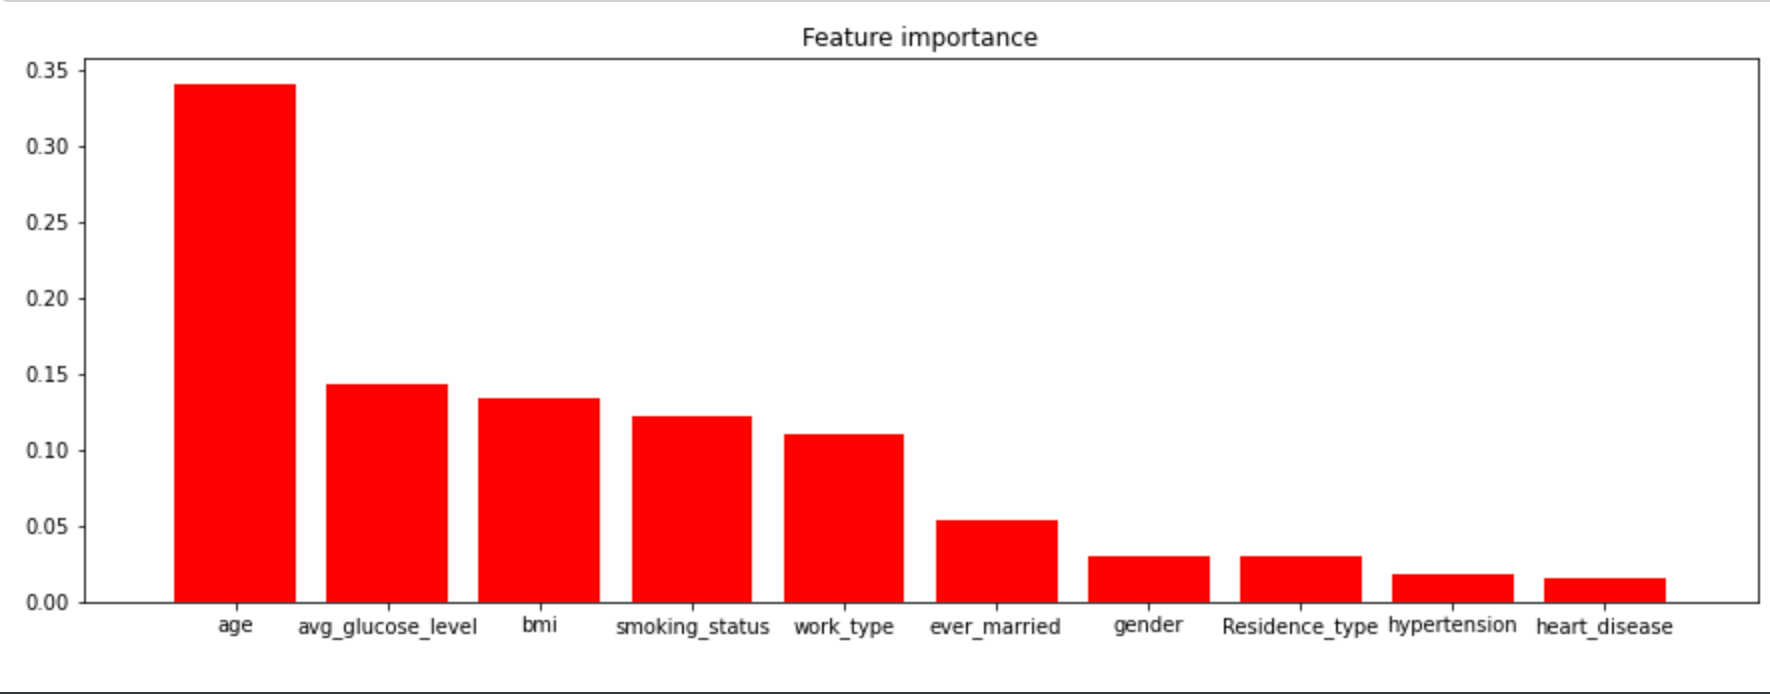
\includegraphics[width=1\linewidth]{Feature_Importances}
    \caption{Feature Importance}
    \label{fig:Figure7}
\end{figure}

\subsection{Future Work}
\label{sec:conclusion: Future Work}


\noindent For future work, we would like to explore the importance of various features to help filter features that are irrelevant or redundant. This would help improve the models which are used to predict whether a patient is likely to have a stroke. In addition, we would like to experiment with finding the optimal learning rate for the stochastic gradient algorithm. Small learning rates tend to converge too slowly, which makes our model too inefficient, whereas large learning rates causes our model to overshoot the minima and diverge. Finding the optimal learning rate will help in lowering the number of iterations in order to find a model with high accuracy.\\

\noindent Some extra conclusions we determined were that, apart from a lot of categories that do not make sense for this context, some of the metrics are flawed. BMI in general is not a good metric to use, so it would be better to measure weight \cite{BMI}. Also, we are unsure if smoking is related to tobacco, cannabis, crack cocaine, or any other drug that can be inflammed and inhaled. Nonetheless, we see that age is clearly the biggest contributor to one's likelihood to suffer a stroke by far.